\chapter{Búsqueda en profundidad (DFS)}
La búsqueda en profundidad, o DFS es un tipo de búsqueda basada en el Backtracking que vimos en el capítulo anterior, lo que la caracteriza es no explorar el mismo lugar dos veces.

El código de una DFS en general se verá de la siguiente forma:

\begin{lstlisting}
	void DFS(estado) {		
		if (estado fue visitado)
			return;
		marca el estado como visitado;
		for (transiciones del estado) {
			DFS(transicion);
		}
	}
\end{lstlisting}

Veamos un problema ejemplo:

\section*{Ejemplo: Dos operaciones}
Javier tiene una calculadora un poco peculiar. Esta tiene un entero \(x\) en la pantalla y dos botones.
\begin{plimits}
	\item El primer botón, al ser presionado le suma \(a\) al número \(x\).
	\item El segundo botón, al ser presionado le suma \(\frac{x}{b}\) a \(x\),  este botón solo puede ser usado cuando \(x\) es múltiplo de \(b\).		
\end{plimits}

Conociendo \(a\) y \(b\), determina si de el valor inicial de \(x\), se puede llegar a tener el número \(y\) en la calculadora.

Además, si se puede imprime como.

\textbf{Entrada}\\
Recibes cuatro enteros \(x\), \(y\), \(a\) y \(b\). El valor inicial de la calculadora, el valor deseado, el valor de a, y de b; respectivamente.

\textbf{Salida}\\
Si es imposible convertir \(x\) en \(y\), deberás imprimir \verb|NO|.

Si es posible, deberás imprimir un entero \(K\) representando en cuantos pulsaciones de botón lo puedes hacer.

En la siguiente línea imprimirás \(K\) enteros, siendo las pulsaciones a los botones que debes hacer en orden de izquierda a derecha. Un \verb|1| es presionar el primer botón, y un \verb|2| representa el segundo botón.

Si hay varias respuestas, imprime cualquiera. (Ojo: no necesitas minimizar \(K\)).

\textbf{Ejemplo}\\
\begin{casebox3}
	\ecase{
		1 20 4 5
	}{
		6\\
		1 2 1 2 1 1
	}{
		Presiona el primer botón, ahora tienes 5.\\		
		Usa el segundo, ahora vale 6.\\
		Pulsa el primer botón, obtienes 10.\\
		Utiliza el segundo para tener 12.\\
		Usa el primer botón, obtén 16.\\
		Termina con el primero, llegamos a 20.
	}
	\ecase{
		1 32 3 2
	} {
		NO
	}{
		Es imposible obtener 32.
	}
\end{casebox3}

\textbf{Límites}
\begin{plimits}
	\item \(1\leq x, y, a, b \leq 10^5\)
\end{plimits}

TODO ENLACE

\subsection*{Solución}
Iniciemos con la fuerza bruta.

Podemos ver que cada paso tenemos que tomar dos decisiones, o usamos el botón 1 o el 2. Podemos hacer una búsqueda exhaustiva para ver cual decisión tomar.

\begin{minipage}{\linewidth}
\begin{lstlisting}
	void exhaustiva(int x, int pasos) {
		if (x==y) {
			cout << pasos<<"\n";
			for (int i =0; i <pasos; i++) {
				cout<<solucion[i]<<" ";
			}			
			exit(0);
		}
		if (x>y) {
			//x solo crece, de aqui ya es imposible hallar a y.
			return;
		}
		//presiona el boton 1.
		solucion[paso]=1;
		exhaustiva(x+a; pasos+1);,
		
		//presiona el boton 2 si es posible.
		if (x%b==0) {
			solucion[paso]=2;
			exhaustiva(x+x/b, pasos+1);
		}
	}
	
	int main() {
		[...]
		exhaustiva(0,0);
		cout << "NO";
	}
\end{lstlisting}
\end{minipage}

Sin embargo, como ya hemos visto, la complejidad de la búsqueda exhaustiva es exponencial, por lo que no correrá para los límites de \(10^5\) que pide este problema. 

Pero, ahora dibujemos lo que hace la búsqueda exhaustiva en el primer caso para ver si podemos mejorarlo.

\begin{center}
	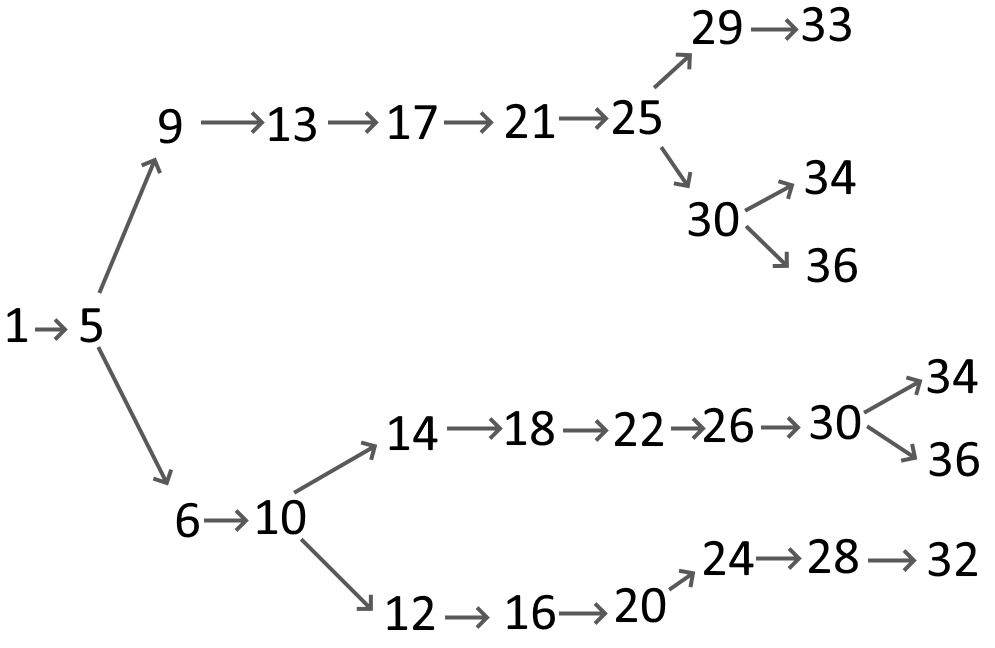
\includegraphics[scale=0.3]{exhaustivaDFS1}
\end{center}

Allí vemos que podemos llegar al 30 con dos rutas. Pero sin importar cual ruta sigamos, de allí solo podemos llegar a los mismos números, al 34 y al 36.

Por lo tanto pregunto ¿realmente tiene sentido la segunda vez revisar el 30?

No, no lo tiene. Al llegar por segunda vez podemos podar la búsqueda, pues ya hemos visto todas las opciones del 30 antes, lo cuál nos ahorrará operaciones. 

Ahora nuestra recursión se vería:
\begin{center}
	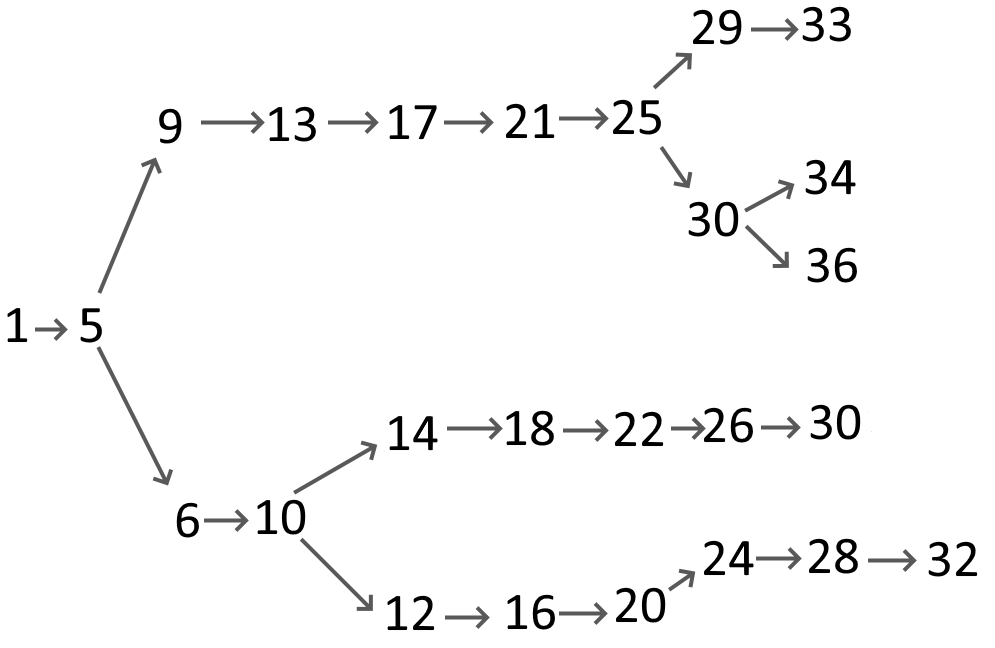
\includegraphics[scale=0.3]{exhaustivaDFS2}
\end{center}

Puede que esto no se vea impresionante en el primer caso ejemplo, pero en el segundo caso ejemplo sí evitamos explorar mucho. Con esta regla, en el segundo ejemplo pasamos de 88 llamadas a la recursión a solo 31.

Entonces, para aplicar la nueva regla podemos tener un arreglo de booleanos llamado \verb|visitado| que lleve cuenta de cuales valores ya visitamos con la búsqueda.

Cuando visitemos un valor de \(x\) revisamos si fue visitado antes, si lo fue detenemos la recursión, si no marcamos a \(x\) como visitado y continuamos con la búsqueda.

Esto en código se ve como:

\begin{minipage}{\linewidth}
\begin{lstlisting}
bool visitado[100005];
void busqueda(int x, int pasos) {
	if (x==y) {
		cout << pasos<<"\n";
		for (int i =0; i <pasos; i++) {
			cout<<solucion[i]<<" ";
		}			
		exit(0);
	}
	if (x>y) {
		//x solo crece, de aqui ya es imposible hayar a y.
		return;
	}
	if (visitado[x]) 
		return;
	visitado[x]=true;
	//presiona el boton 1.
	solucion[paso]=1;
	busqueda(x+a; pasos+1);,
	
	//presiona el boton 2 si es posible.
	if (x%b==0) {
		solucion[paso]=2;
		busqueda(x+x/b, pasos+1);
	}
}

int main() {
	[...]
	busqueda(0,0);
	cout << "NO";
}
\end{lstlisting}
\end{minipage}

Y tal cual, esto es una DFS, una búsqueda que va probando todas las opciones de donde se encuentra actualmente, pero nunca repitiendo la búsqueda en lugares ya visitados.

Analicemos la complejidad de este algoritmo, aquí es donde esta lo genial de este tema.

Veamos que este código solo ejecuta la parte de probar al botón 1 y 2 una sola vez por cada valor de \(x\) posible.

Y la parte de arriba solo es ejecutada tantas veces como búsqueda sea llamada(), que ya vimos que esta limitada a los posibles valores de \(x\).

Como nuestros valores de \(x\) varían desde \(1\) hasta \(y\), la complejidad de este algoritmo es \(O(y)\). Lo cual significa que pasamos de un algoritmo exponencial a uno lineal. He aquí la hermosura de la búsqueda en profundidad, o DFS.

\section{Estados y transiciones}
Para entender completamente la DFS necesitamos definir un poco más sobre lo que explora.

En vez de llamar al valor de \(x\) que llevamos en la búsqueda como ``lugar", o cualquier otra cosa, ahora le llamaremos por su nombre más formal de estado.

Y las ``opciones" que tenemos en cada decisión le llamaremos por su nombre correcto, transiciones.

De forma que la DFS explora un espacio que esta conformado por estados conectados entre ellos por transiciones. Cada estado tendrá sus transiciones que nos permitirán alcanzar a otros estados.

En el código recursivo que hemos hecho de DFS, los estados vienen en los argumentos de la recursión y las transiciones son las llamadas recursivas que hacemos.

Entonces, nuestra búsqueda DFS explora todos los estados alcanzables desde uno inicial, utilizando las transiciones disponibles para pasar de estado a estado.

\section{Complejidad}
La complejidad de una DFS es la cantidad de estados más transiciones, llamemos al número de estados \(V\) y \(E\) al número de transiciones total. La DFS corre en \(O(V+E)\).

En el ejemplo anterior teníamos \(y\) estados, así como a lo más \(2y\) transiciones (dos por cada estado de los botones), la complejidad del ejemplo es pues: \(O(V+E)=O(y+2y)=O(y)\).

\section*{Problemas de práctica}
\addcontentsline{toc}{section}{Problemas de práctica}

\begin{exercise}
	\problema{Subiendo la torre II}{TODO}
\end{exercise}

\begin{exercise}
	\problema{Camino en la matriz}{TODO}
\end{exercise}

\begin{exercise}
\problema{Lugares alcanzables}{TODO}
\end{exercise}
